\documentclass{article}
\usepackage[utf8]{inputenc}
\usepackage[margin=80pt]{geometry}
\usepackage{amssymb}
\usepackage{amsmath}
\usepackage{enumitem}
\usepackage{graphicx}
\usepackage{algorithmic}
\usepackage[table,xcdraw]{xcolor}
\usepackage[hidelinks]{hyperref}

\begin{document}
\tableofcontents
\newpage
\section{Introduction}
This section aims to clarify the goal of the project, as well as describing the philosophy and the tools used by this team to efficiently collaborate and achieve better results. In addition, any assunmptions made about the project are reported and a short description of the all content is given.
\subsection{Goal of the project}
Given the description of a software application, an e-broker\footnote{An e-broker is a brokerage house that allows you to buy and sell stocks and obtain investment information from its Web site} system, use a variety of diagrams(UML, dataflow etc.) in order to better analyze the requirements, functional or not, of the application. 
\subsection{How we worked}

\subsubsection{Trello}
To better collaborate and organize our work, we used \href{https://trello.com}{\underline{\textit{Trello}}}, a flexible project management tool, by assigning weekly tasks to each member of the team.

\subsubsection{Git}
In order to exploit work parallelism, while keeping track of all progress the rest of the team made in the meantime, we used the famous VSC \href{https://github.com/}{\underline{\emph{git}}}\footnote{One can take a look at the source code of this project or even contribute, \href{https://github.com/KostasKoyias/Software_Analysis}{\underline{\textit{here}}}} using \href{https://nvie.com/files/Git-branching-model.pdf}{\underline{\emph{this}}} branching model. For those unfamiliar with git, it is a distributed version-control system, tracking changes in source code during software development to better coordinate work among programmers. Whenever a task was completed, the corresponding member requested a review. Then, the rest of the team was able to review the set of changes, discuss potential modifications, or even enhance the commit. Eventually, in most cases, the request was approved and merged into the main branch.

\subsubsection{Discord}
As in every team project, in order to optimize performance, meetings really were a necessity. We sure had some face-to-face meetings, but that was not always possible. So, another tool we used is \href{https://discordapp.com/}{\underline{\emph{Discord}}}, a platform designed for video gaming communities, that specializes in text, image, video and audio communication between users in a chat channel. Using Discord's video-chatting and screen-sharing features helped us co-ordinate and co-operate easy and fast. As a team, we agreed on having short but frequent meetings(2 or 3, 10 minute meetings per day) in order to take full advantage of time, optimizing performance in general.

\subsection{Submission}
Work load was pretty well distributed amongst all members of this team throughout the whole process of deployment. The one member responsible of reviewing the final version of this pdf and submitting it to e-class is
\href{https://github.com/KostasKoyias}{\emph{Konstantinos Koyias}}.  

\subsection{Assumptions}
Despite the detailed and informative description of the project, there were a few points we had to intervene, make our own assumptions and decide on what is best to follow. The most important of those were:
\begin{itemize}
\item 
\item
\end{itemize} 

\subsection{Chapters} 

\subsubsection{Structured Analysis}
This chapter contains:
\begin{itemize}
\item The dataflow diagram of the e-Broker system.
\item Dataflow diagrams for levels 1 and 2 of procedure decomposition.
\item The process decomposition tree.
\item Specifications for:
\begin{enumerate}
\item The process of transmitting order in Structured English.
\item The process of supply estimation using a Decision Table.
\item The process of a client's log in the e-Broker system using a Tree.
\item Removing a command from the Data Dictionary.  
\end{enumerate}
\end{itemize} 

\subsubsection{UML}
In this chapter, we used the general-purpose, developmental, modeling language UML in order to visualize the design of the e-Broker system. Specifically, the following were included:

\begin{itemize}[{label=\tiny$\triangleright$}]
\item Use Case diagram of the system.
\item Class diagram of the system.
\item State-machine diagram of the entity ``Command''.
\end{itemize}

To better model the stock selling/buying operations we included:

\begin{itemize}[{label=\tiny$\triangleright$}]
\item A main success case Scenario and some alternative ones.
\item An Activity diagram.
\item A detailed Class diagram.
\item A Sequence Diagram.
\item A Communication Diagram.
\end{itemize}

\subsubsection{Structured Design}
This is the chapter where a systematic methodology using
\begin{itemize}
\item a Programm Structure diagram and 
\item a piece of pseudo-code that formulates the control unit of
\begin{itemize}[{label=$\circ$}]
\item the main transformation 
\item the M3 transformation 
\item the M4 transformation
\end{itemize}
and the presentation unit of
\begin{itemize}[{label=$\circ$}]
\item the M2 transformation 
\end{itemize}
for the corresponfing Programm Structure diagram.
\end{itemize}
determines the design specifications of the application. 

\newpage
\section{Structured Analysis}
\subsection{e-Broker Dataflow diagram}
a

\subsection{Procedure decomposition Dataflow diagrams}
b

\subsection{Process decomposition Tree}
c

\subsection{Specifications}
In this section, each specification is examined separately using a variety of Structured Analysis tools. 

\subsubsection{Transmitting Order}
Using Structured English, the Transmitting Order process from the e-Broker system point of view looks as follows:\\
\begin{algorithmic}[H]
 \WHILE{Form Is Invalid OR Customer is Re-editing}
  	\STATE Display Form
  	\STATE On Submit do
  	\IF{Form Is Incomplete}
  		\STATE Display ``All fields required" message
   
    \ELSIF{There is Field with Invalid Type}
  		\STATE Display ``Invalid field value" message
  	\ELSE
  		\STATE Display Preview
  		\STATE Display ``Back to Editing?" message
  	\ENDIF
 \ENDWHILE
 \STATE Forward command to A.S.T
 \STATE Get response
 \IF{Response is negative}
  	\STATE Display ``Rejected" message
 \ELSE
  	\STATE Display ``Approved" message
 \ENDIF

\end{algorithmic}

\subsubsection{Supply Estimation}
In this little section, we will use a decision table in order to help us simplify the complex process of calculating the exact charge of a Customer for a transaction.
\begin{table}[htbp]
\begin{tabular}{|l|l|l|l|}
\hline
\rowcolor[HTML]{EFEFEF} 
\textbf{Conditions} & Rule 1               & Rule 2               & Rule 3               \\ \hline
Volume              & $0 - O_1$            & $O_1-O_2$            & $O_2-O_3$            \\ \hline
\rowcolor[HTML]{EFEFEF} 
\multicolumn{4}{|l|}{\cellcolor[HTML]{EFEFEF}\textbf{Actions}}                           \\ \hline
Set charge equal to & $P_1$\% $\times Volume$ & $P_2$\% $\times Volume$ & $P_3$\% $\times Volume$ \\ \hline
\end{tabular}
\end{table}

\subsubsection{Log in}
Authentication is not always simple.\\
This is a detailed \textbf{decision tree} that proves just that.\\
\hspace*{5mm}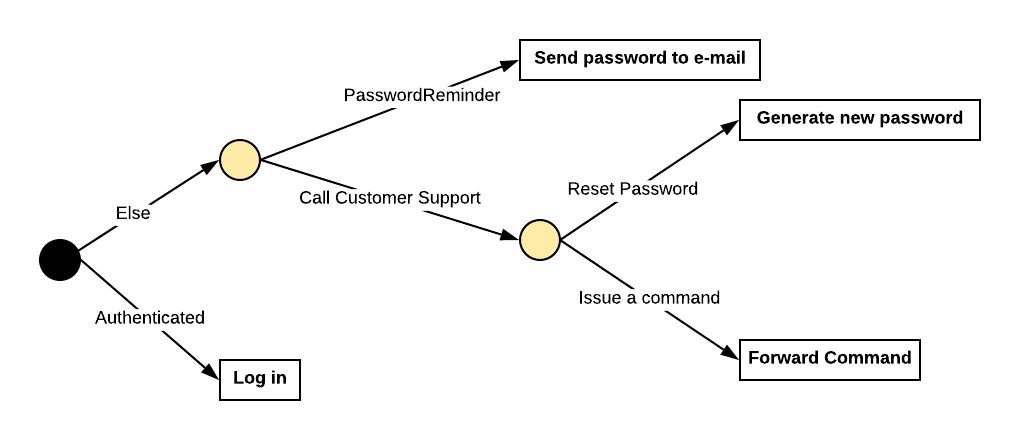
\includegraphics[scale=0.4]{decisionTree} 

\subsubsection{Data dictionary of Command Report}
dd

\newpage
\section{UML}
In this chapter, all neccessary UML diagrams for the e-Broker system will be created. In order to distinquish relationship types, we used this map: \\\hspace*{16mm}\{always: include, might: extend, generic: generalization\}. \\
This gets a bit more clear in the following subsection. 
\subsection{Use Cases}
After taking a good look at the description of the system, we came up with the following actors:
\begin{itemize}
\item Customer(Primary)
\item Customer Support Department(Secondary)
\item Athens Stock Exchange(Secondary)
\end{itemize}
 and the corresponding use cases. Each customer can:
\begin{itemize}
\item \textbf{log in}\\This action will \textbf{always} trigger a password check, and it 
\textbf{might} lead to an error message. In this case a \textbf{generic} ``forgot password'' request \textbf{might} happen, which can be either a password reminder via an e-mail, or a call to the \textit{C.S.D} for a new password or/and a command to be executed.
\item \textbf{command}\\A \textbf{generic} command, can be either a creation or a cancellation, both of which will \textbf{always} have to be reviewed by the \textit{A.S.E}. This \textbf{generic} review will either lead to an approval or a rejection. An approved command \textbf{might} at some point get cancelled, otherwise the \textit{Customer} will 
\item \textbf{get a report}
\end{itemize}
so we came up with the following use case diagram\\
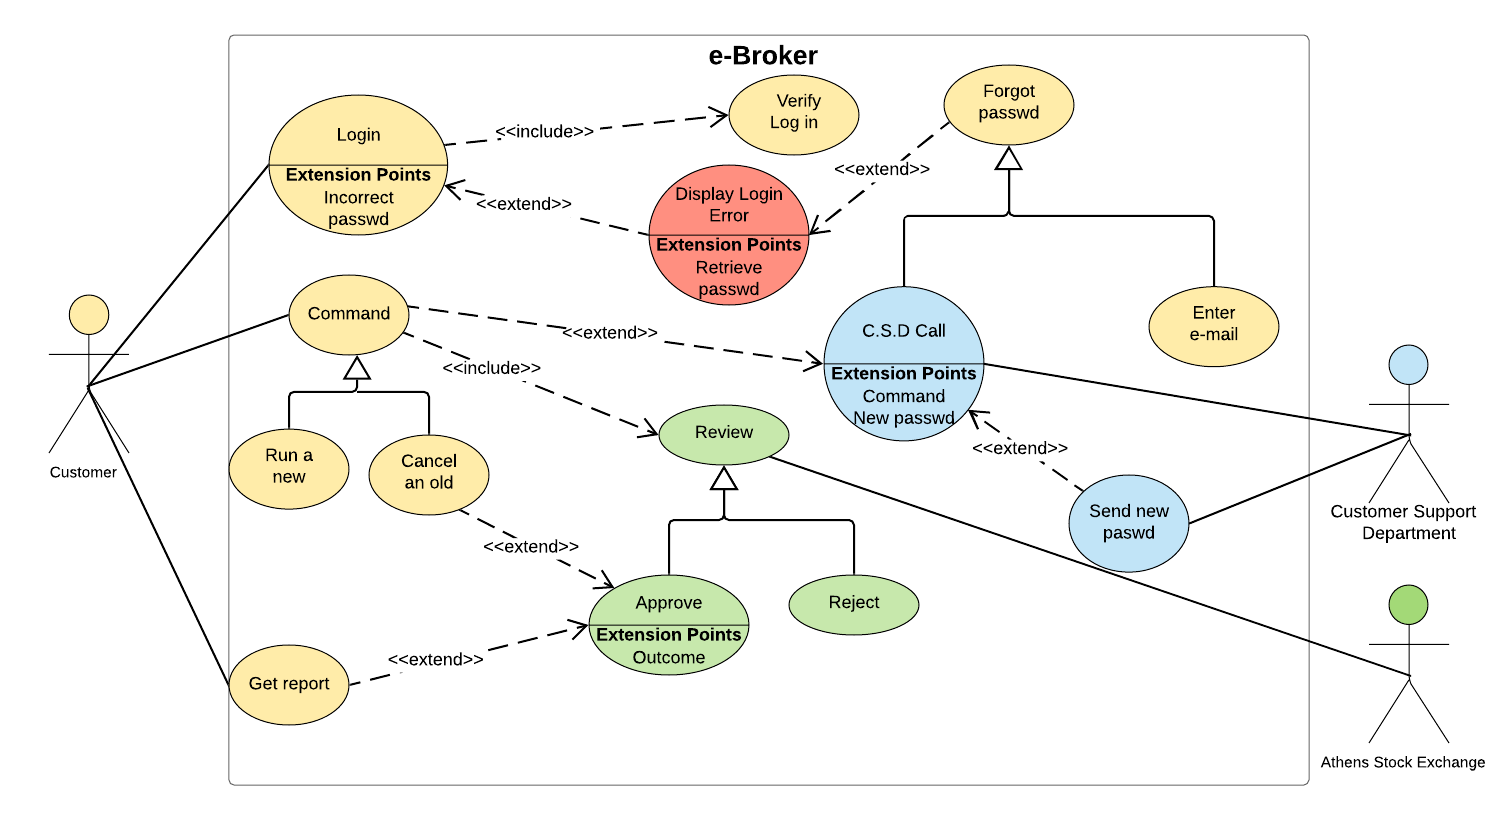
\includegraphics[scale=0.3]{use_cases}

\newpage
\subsection{Classes}
This is the section, where classification took place. Notice that C.S.D and A.S.E are just objects, like instances, not classes, so they have no place in the following diagram.\\
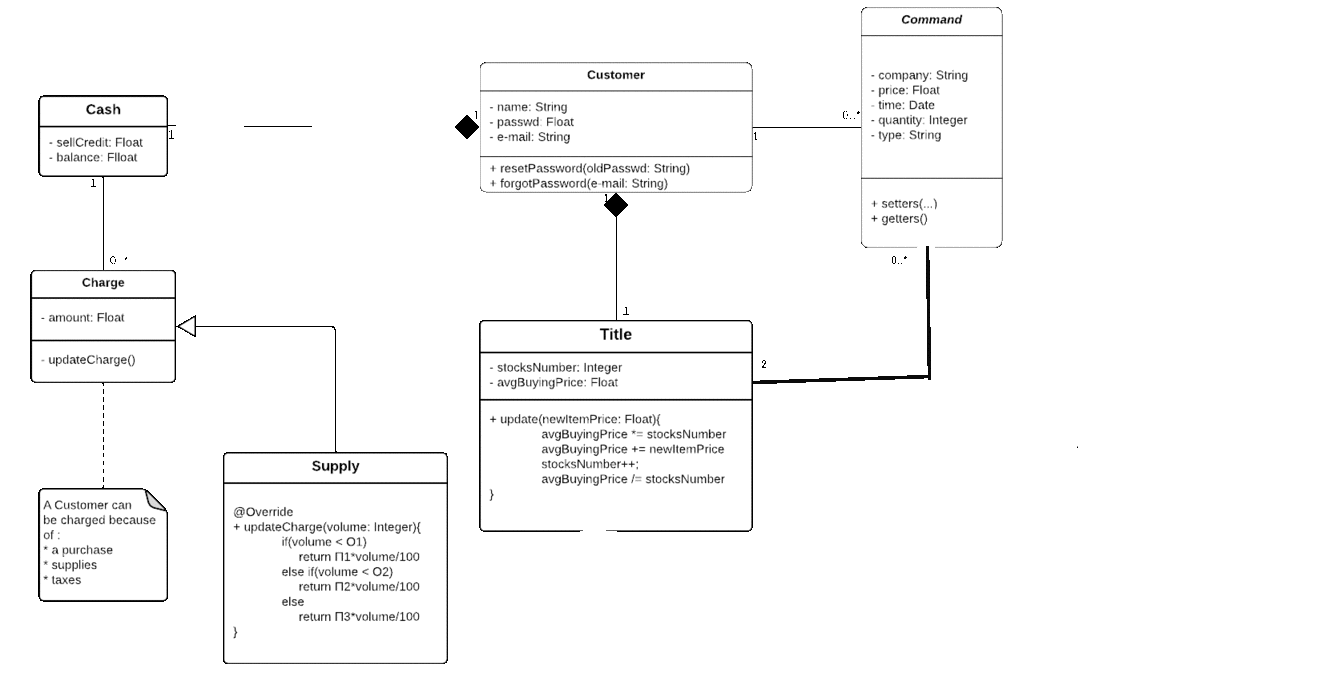
\includegraphics[scale=0.3]{classesII}\\
Let us now explain what is happening on the diagram above.\\
\begin{itemize}
\item First off, some data is kept for each \textbf{Customer}, a \textbf{Cash} and a \textbf{Title}. 
These, can not really exist without a Customer. 
This is called composition and we used a black diamond to denote it.
\item Each Customer is able to request for as many \textbf{Command}s as he wishes, if any, to be executed or cancelled.
\item Each Command, is associated with exactly two(2) Titles, one of them belongs to the buyer and the other, to the seller. 
\end{itemize}
Notice that we could use three extra classes extending \textbf{Charge}, namely Purchase, Supply and Tax but other than Supply, a class with a different updateCharge aproach, all of them would not add any attribute or method up to their parent, so we decide not to define classes Purchase and Tax. Lastly, to avoid a huge diagram we omitted the following fields of Customer:\\  
fathername, mothername, address, birthDate, id, tax{\_}id and financialService.
   
\newpage
\subsection{Command Lifecycle}
By reading the description of the system, one might notice that the lifetime of the \emph{command} entity happens to be a realy interesting one. Well, in that case, a common technique is using a state-machine diagram to better visualize all possible outcomes of feature.\\
For a command to be executed, all properties it has, need to first be defined using a form.\\
After a successful submission, meaning all fields contain values of the right type, the command will be reviewed. In case of an approval, it will be executed as soon as possible. In the meantime, it can be cancelled. But, this in only possible in case of an independent command, meaning it has no recursive effect to any previously executed commands, because they can not be reverted now in any way. The diagram follows:\\
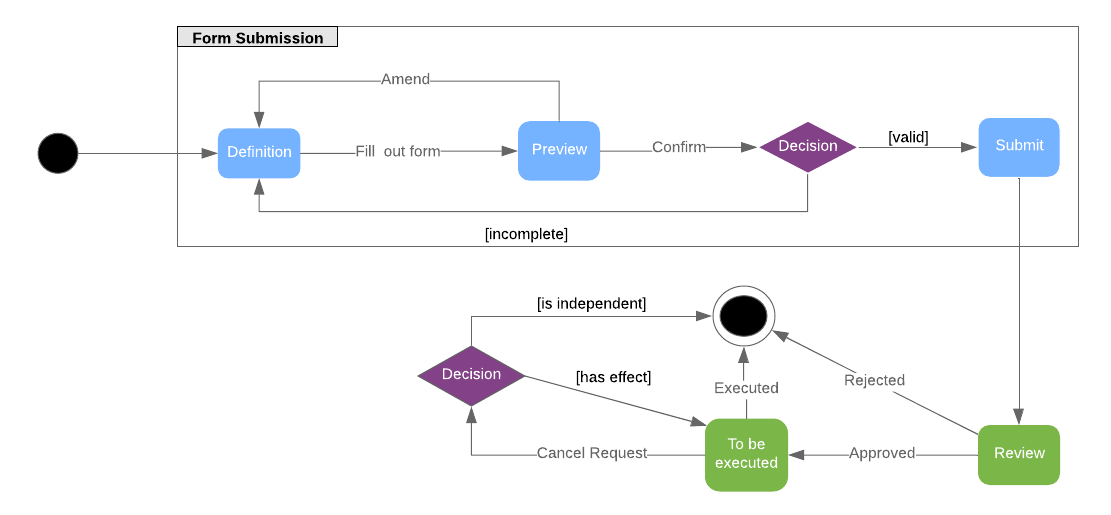
\includegraphics[scale=0.325]{state}  

\subsection{Command Transmission}

\subsubsection{Scenarios}
The transmission of a command, although it looks pretty straightforward, is actually a complex one. Let us take a closer look at it step-by-step in order to detect all points where something could go wrong and think about what happens in each of those cases. Steps should look as follows:\\
\begin{enumerate}
\item Customer fills out all attributes of the form
\begin{enumerate}
\item an incomplete form or
\item a field set with a non-matching type or out of range value\\(e.g ``name'' set to an integer, ``time-target'' refers to the past etc.) 
\end{enumerate} 
will take us back to step 1 
\item Customer previews the form
\begin{enumerate}
\item customer decides to modify some field, back to step 1
\end{enumerate}
\item Customer confirms and submits
\begin{enumerate}
\item a network partition occurs, action depends on system availability policy(e.g PACELC, PAVEL etc.) 
\end{enumerate}
\item A.S.C receives request
\begin{enumerate}
\item command execution is not possible, then command is rejected
\end{enumerate}
\item A.S.C approves request, pushes command in the ``To be executed'' priority queue of e-Broker 
\end{enumerate} 

\subsubsection{Activity Diagram}
Once a Customer wishes to execute a command, a form to fill out opens up. It is not until it is complete and contains data of the right type, that the customer can preview it, perhaps request changes and then move on to submit it. At this point the A.S.T receives the submitted form, confirms of receiving it(now the customer is able to parallelly issue another command) and proceed with reviewing it. That will either lead to an approval or a rejection. The exact diagram follows:\\
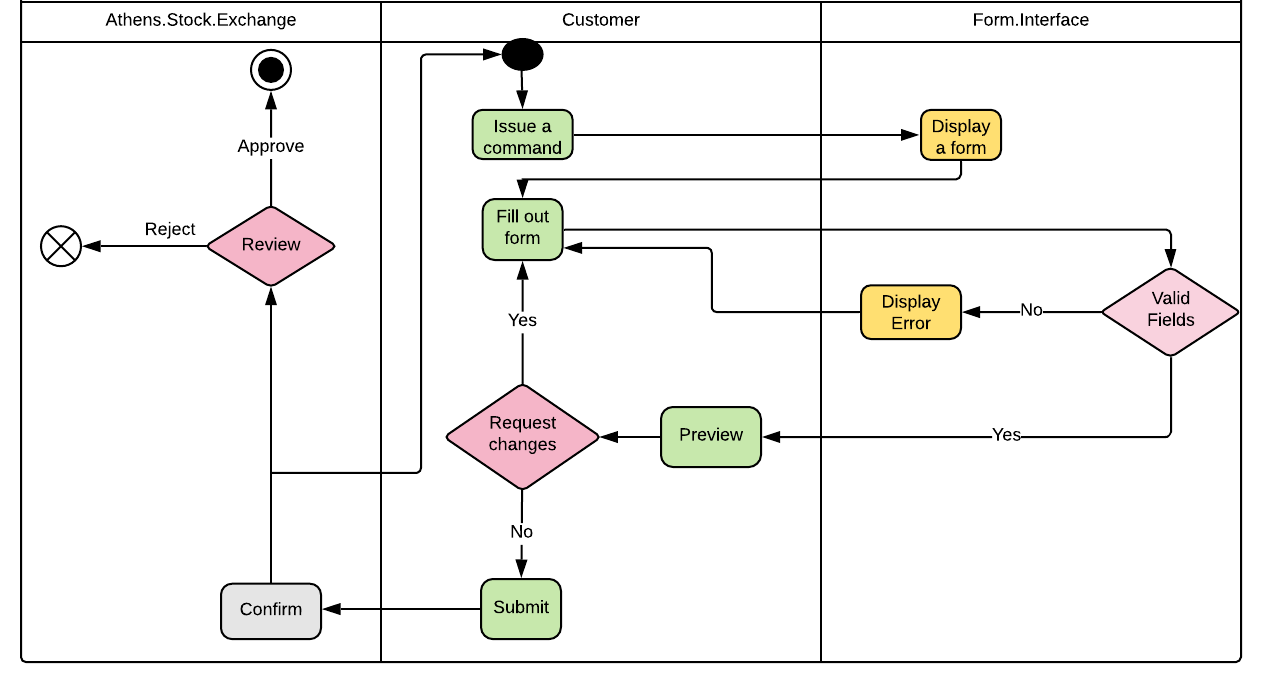
\includegraphics[scale=0.6]{activity}    

\subsubsection{Detailed Class Diagram}
Now, let us take a closer, more detailed look at all classes interacting during the Command phase as well as the
messages exchanged amongst them.\\
\hspace*{25mm}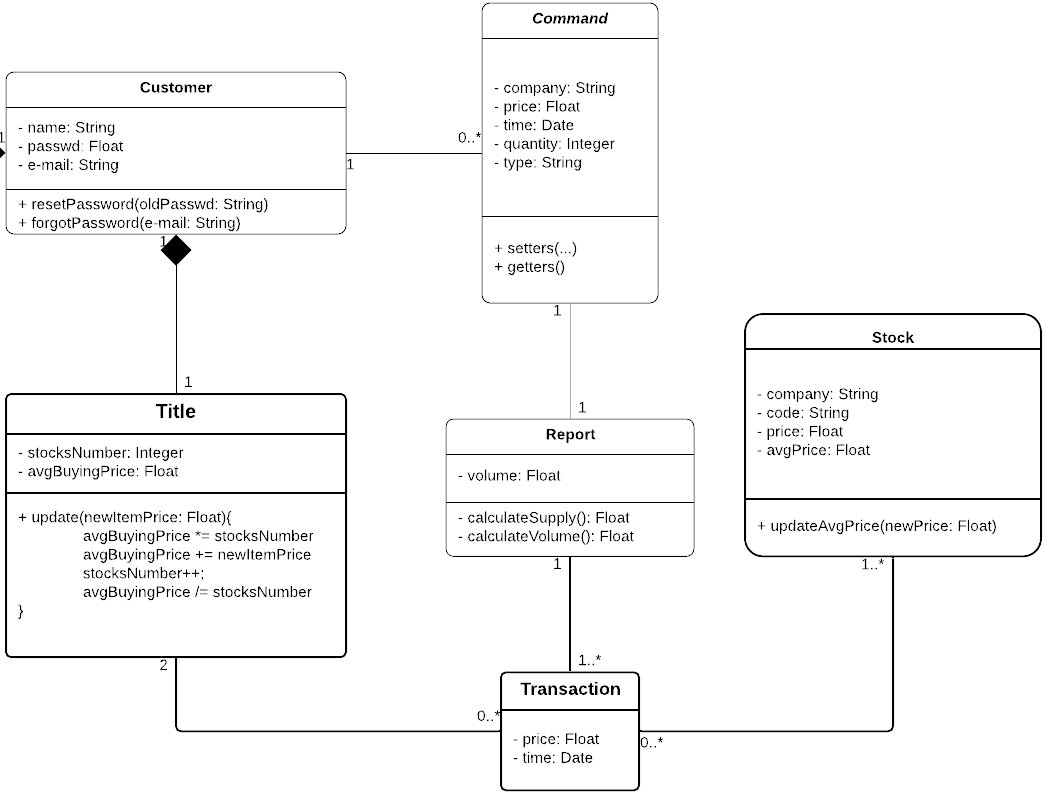
\includegraphics[scale=0.3]{detailed_classes}\\
As we mentioned above, C.S.D and A.S.E are not classes, but just an instance of one, so they are omitted.\\
The above diagram tells us that for each Command, there is a unique \textbf{Report}, associated with at least one(1) \textbf{Transaction} that involves at least one(1) \textbf{Stock} and is associated with exactly two(2) Titles, one for the buyer and one for the seller.
So, a complete and very detailed class diagramm would look like this\\
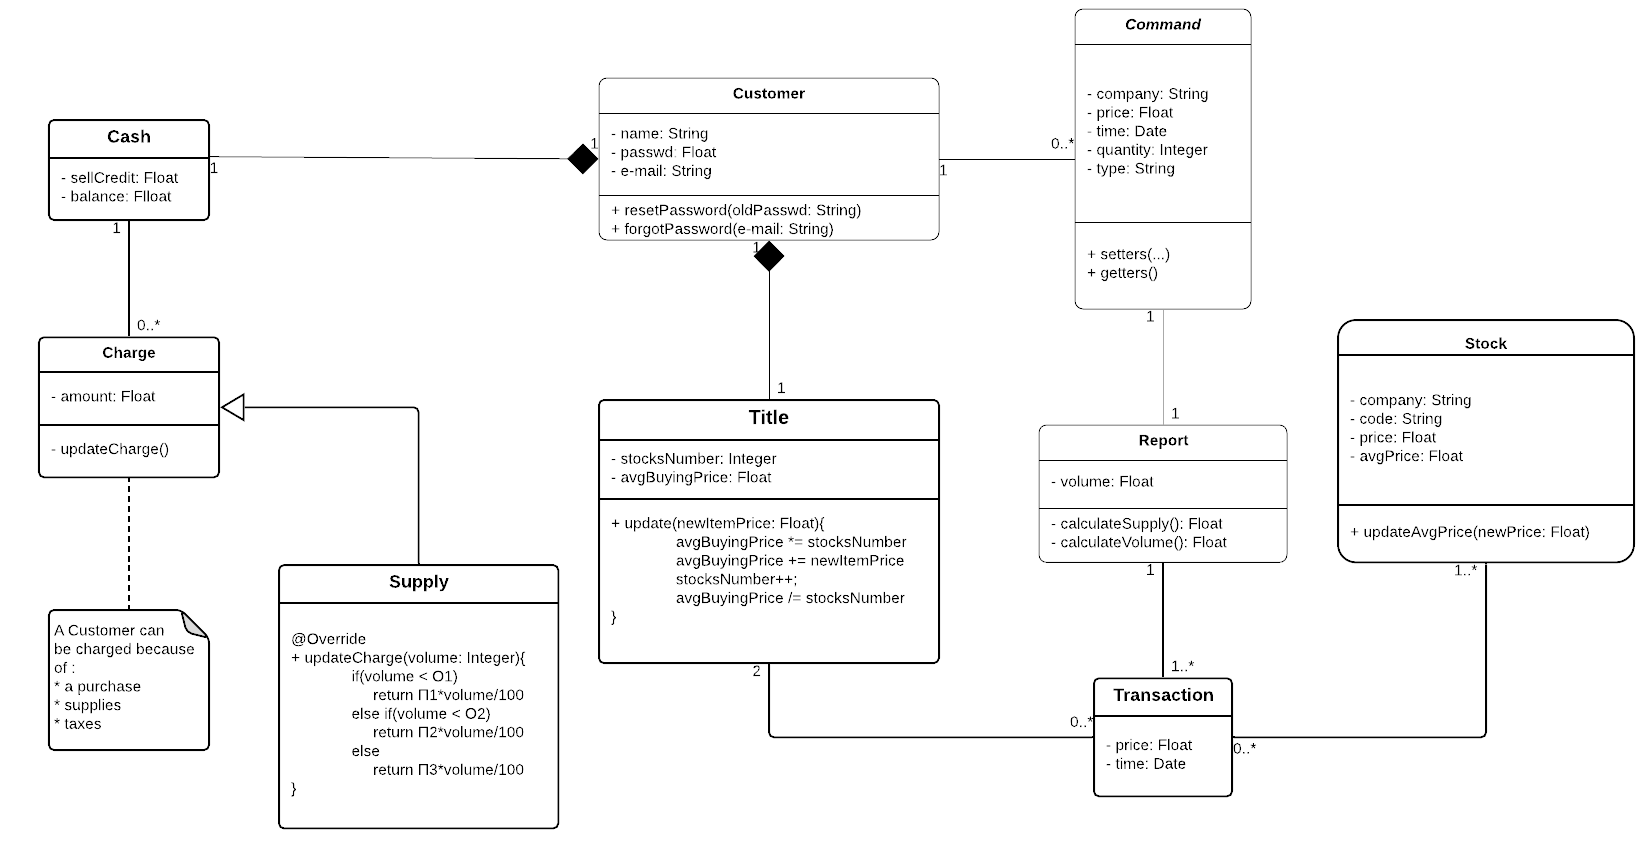
\includegraphics[scale=0.25]{classes}

\subsubsection{Sequence Diagram}
This diagram, in contrast to the Activity one above, analyzes a single scenario from a slightly different scope, using a closer to the implementation approach, intended for the development team to use.\\ 
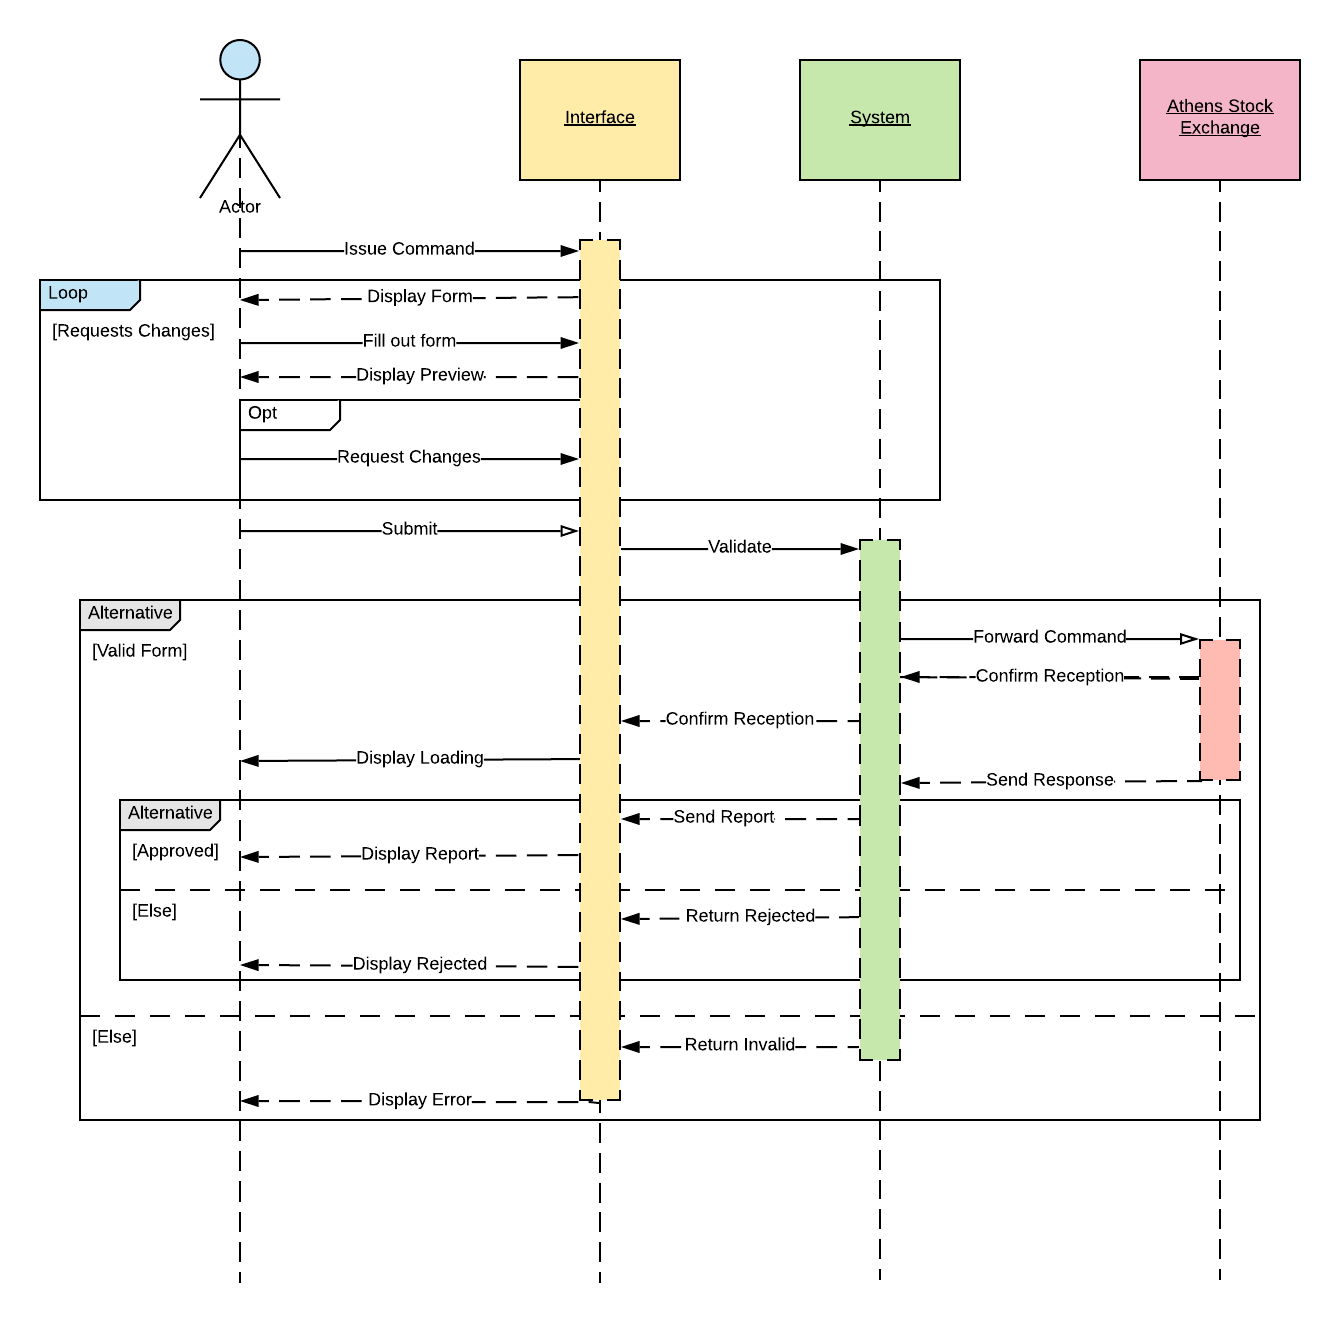
\includegraphics[scale=0.25]{sequence}\\
As you might did notice, a solid line denotes a request, while a dashed line denotes a response. Lastly, open arrow heads were used for asynchronous requests, notice that a Customer is able to carry on after submission and the System will, obviously, not freeze until the Athens Stock Exchange responds after a Customer's command.

\subsubsection{Communication Diagram}
Now, let us focus on object relationships, rather than the sequence of the messages exchanged amongst them.\\
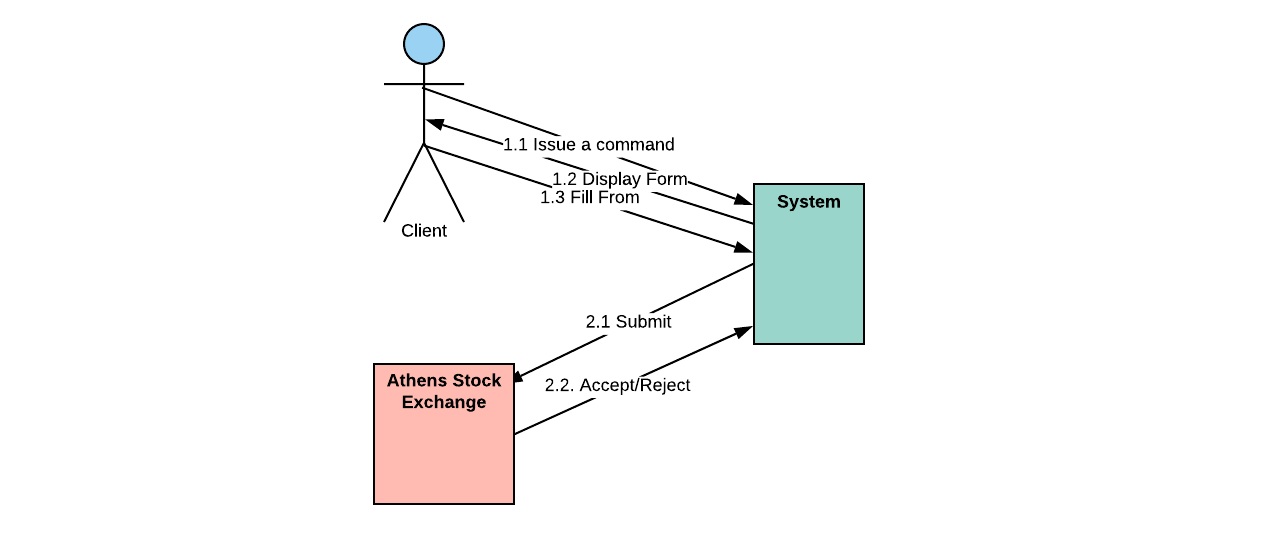
\includegraphics[scale=0.7]{communication}\\

\section{Structured Design}
In this section, we attempted to better determine the design specifications of e-Broker by creating a Program Structure diagram and using pseudocode to better illustrate the functionality of some vital procedures for this application. 
\subsection{From Dataflow diagram to{\\} Program Structure diagram}
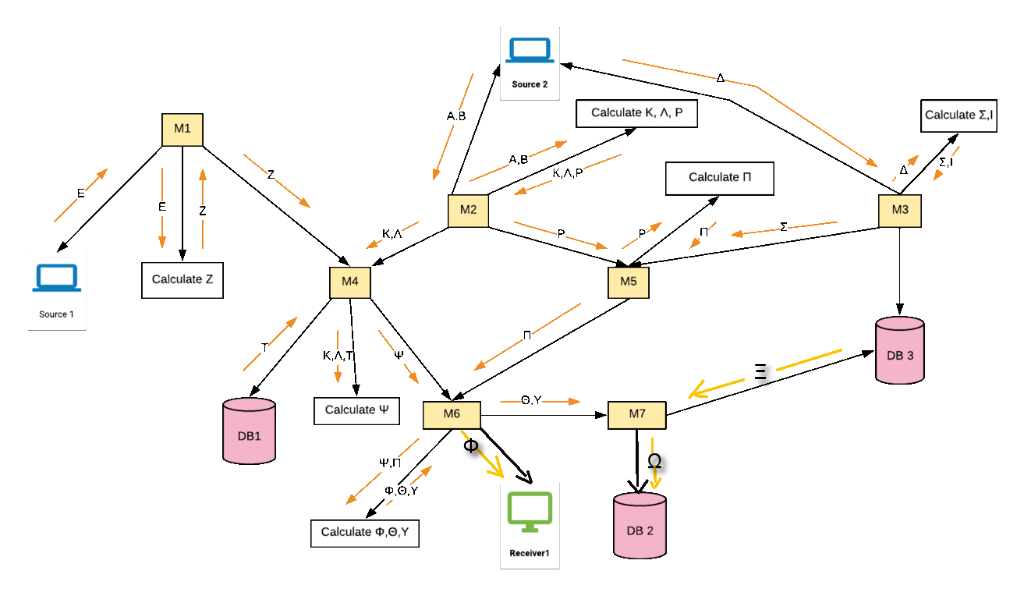
\includegraphics[scale=0.6]{program-structure}

\subsection{Pseudocode Representation of Units}

\subsubsection{Central Transformation}
\begin{algorithmic}[H]
\STATE \underline{\textbf{PROCEDURE M2\_M4}}
	\STATE LOCAL\_VAR T, Z, K, $\Lambda, P, \Psi, \Pi, \Sigma$ 
	\STATE INITIALIZE T, Z, K, $\Lambda, P, \Psi, \Pi, \Sigma$ 
	\STATE EXEC\_M1(Z)
	\STATE EXEC\_M2(K, $\Lambda$, P)
	\STATE GET\_T(T)
	\STATE CALL\_M4(Z, K, $\Lambda, \Psi$)
	\STATE CALL\_M5(P, $\Pi, \Sigma$)
	\STATE EXEC\_M6($\Psi, \Pi$)
\STATE END\_PROCEDURE
\end{algorithmic}

\subsubsection{M3 Transformation Control Unit}
\begin{algorithmic}[H]
\STATE \underline{\textbf{PROCEDURE M3}}(OUT: $\Sigma$)
	\STATE LOCAL\_VAR $\Delta$, I, $\Sigma$
	\STATE INITIALIZE $\Delta$, I, $\Sigma$ 
	\STATE GET\_$\Delta(\Delta)$
	\STATE CALL CALC\_M3($\Delta$, I, $\Sigma$)
	\STATE PUT\_I(I)
\STATE END\_PROCEDURE
\end{algorithmic}

\subsubsection{M4 Transformation Calculation Unit}
\begin{algorithmic}[H]
\STATE \underline{\textbf{PROCEDURE CALC\_M4}}(IN: Z, K, T , $\Lambda$, IN/OUT: $\Psi$)
	\STATE ...
	\STATE //calculate $\Psi$
	\STATE ...
\STATE END\_PROCEDURE
\end{algorithmic}

\subsubsection{M2 Transformation Presentation Unit}
The presentation unit of a trasnforamtion is the one component, responsible of communicating with all users
and external devices/systems. As one can see, M2 is only communicating with one external device, Source 2.
So, the pseudocode for the Presentation Unit of M2 looks as follows:
\begin{algorithmic}[H]
\STATE \underline{\textbf{PROCEDURE GET\_M2}}(IN/OUT: A, B)
	\STATE read A, B from Source\_2
\STATE END\_PROCEDURE
\end{algorithmic}

\newpage
\section{Epilogue}

\subsection{Using Structured Analysis}  
\paragraph{}
Looking back at the Structured Analysis chapter, one might realize that
a graphical represantation of a complex system can be very enlightening and informative both for
a user and for a designer. This is what makes Structured Analysis a great tool, not just for software developmnet, but any
kind of system analysis. To be more precise, in our case, e-Broker is pretty complex at first glance,
but data-flow diagrams manage
to give a clear picture of the system flow by dividing each process as much as needed in order to make the whole concept
easily understandable by not only a designer but a common user as well. Therefore, Structured Analysis is definately a tool
that we are going to use to decompose any complex project that we are assigned in the future, isolating each component of
the system. This will definately make development an easier and much more eenjoyable process. 

\subsection{Working with UML}
Being CS students, using object-oriented languages like, for instance, C++ and Java, is pretty much a common case.
That familiarity helped us absorb the whole usage and syntax of UML rather quickly. This why UML follows the
object oriented concept in the first place. However, it did not take long to notice that UML is a lot more
complex than it looks at first sight. Supporting a variety of different diagrams it was really hard to
express ourselves and describe the same system over and over again from diffent aspects.
One thing we realized using these tools is that avoiding too much detail is a
pretty good idea. These are high-level tools, allowing us to grasp the concept and philosophy of a system, not
the exact implementation. So, \textbf{KISS}(keep it simple stupid) would be our advice to anyone new to UML,
trying to be as precise as possible, omitting exhaustive details which are entailed by the rest of the context
and anyone can figure is what you want. 
 

\subsection{Conclusion}
To sum things up, UML feels more natural to a software developer in contrast to Structured Analysis that seems
to be the perfect fit for simple users to understand how a complex system works taking a really high-level look
at the systems' components. As CS it is rather natural to go with UML. However, I think that Structured Analysis,
a more simple approach to system analysis, is what we would rather use for projects that are not too large.

\end{document}